% Section content template for individual Educative lessons
% This file contains the actual content for a specific section
% Generated from Educative API section content

% Section: Class Diagram for Stack Overflow
% Section ID: 5490973346103296
% Section Slug: class-diagram-for-stack-overflow
% Generated: 2025-12-12T22:50:09.034368

In this lesson, we'll identify and design the classes, abstract classes, and interfaces based on the requirements we have previously gathered from the interviewer in our Stack Overflow system.

\subsection{Components of Stack Overflow}\label{FZNSAv7BINzBDXcttnPa1}
\\
As mentioned earlier, we will design the Stack Overflow system using a bottom-up approach.

\subsubsection{Guest}\label{i8U2Vc6cG1EfBJNe4iJZ7}
\\
The \texttt{Guest} class is a user who can only search and view questions and their answers.
\\
The visual representation of the \texttt{Guest} class is provided below:

\begin{figure}[htbp]
 \centering
 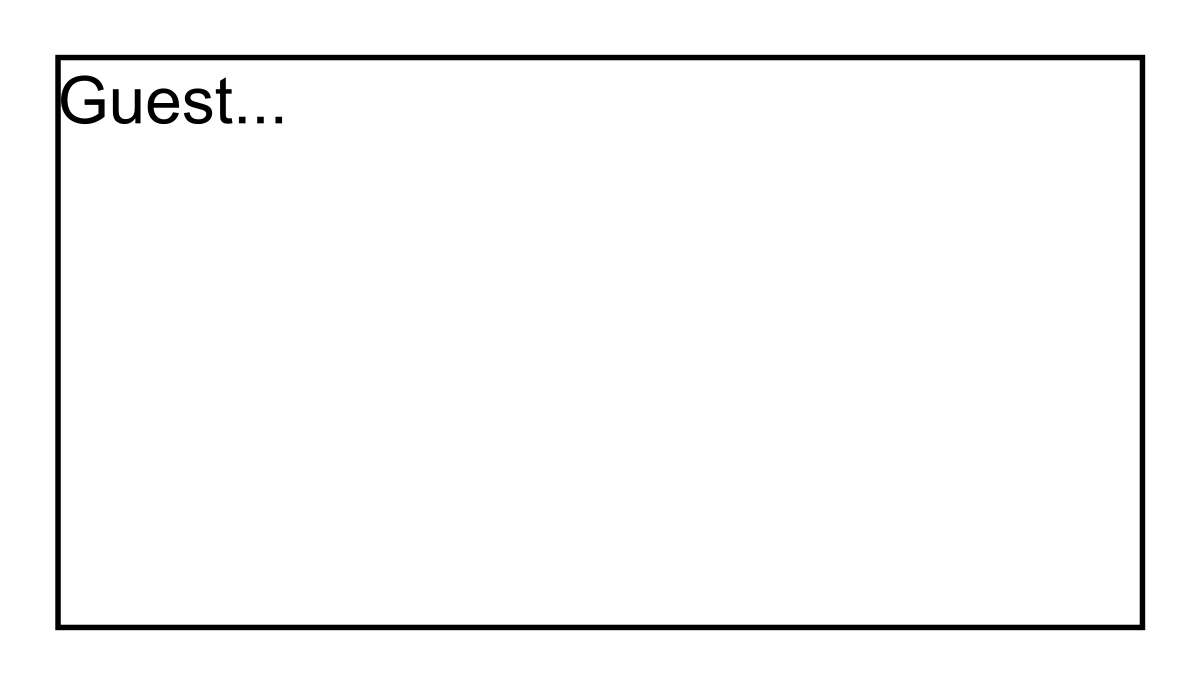
\includegraphics[width=0.5\textwidth]{Images/chapter_20/section_5490973346103296/6284618037592064.png}
 \caption{The class diagram of the Guest class}
\end{figure}

\textbf{R1:} Any guest can view questions and search questions by tag, username, or words

\subsubsection{Question}\label{hFzZET3RCxEY7x8Pc--ri}
\\
The \texttt{Question} class is used to enter the details of the question being asked by a user, such as its title, content, tags, etc. It can also allow users to add comments and bounties.
\\
Here is what the class definition looks like:

\begin{figure}[htbp]
 \centering
 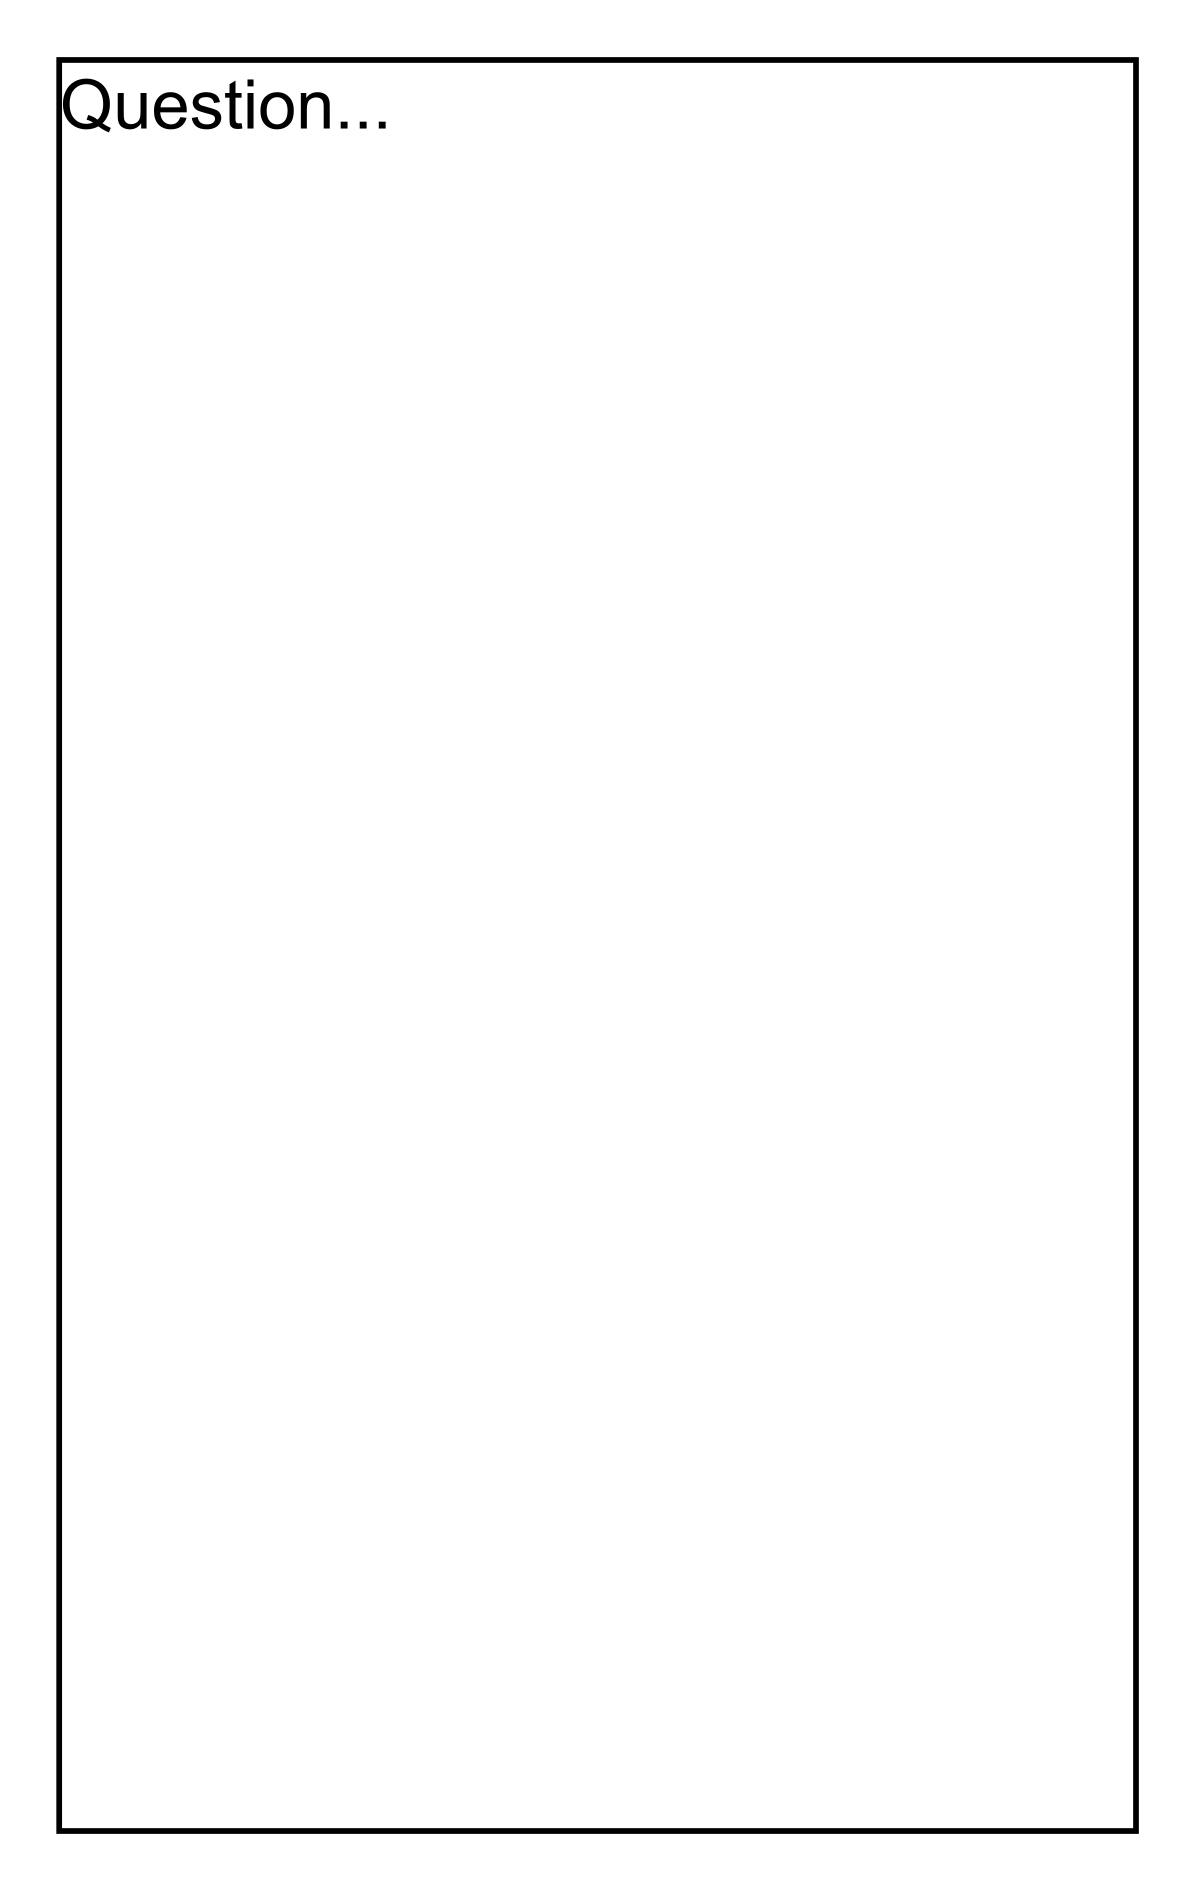
\includegraphics[width=0.5\textwidth]{Images/chapter_20/section_5490973346103296/4792321475215360.png}
 \caption{The class diagram of the Question class}
\end{figure}

\textbf{R2:} Users should be able to post new questions and add answers to an open question.
\\
\textbf{R4:} A user can upvote, downvote, and add comments to a question or answer, while they can only upvote a comment.

\subsubsection{Answer}\label{jxlsCJS3IuU4OE5PDMCpr}
\\
The \texttt{Answer} class represents a user's answer to a question and will contain elements like content, upvotes, and downvotes.
\\
The UML representation of the class is shown below:

\begin{figure}[htbp]
 \centering
 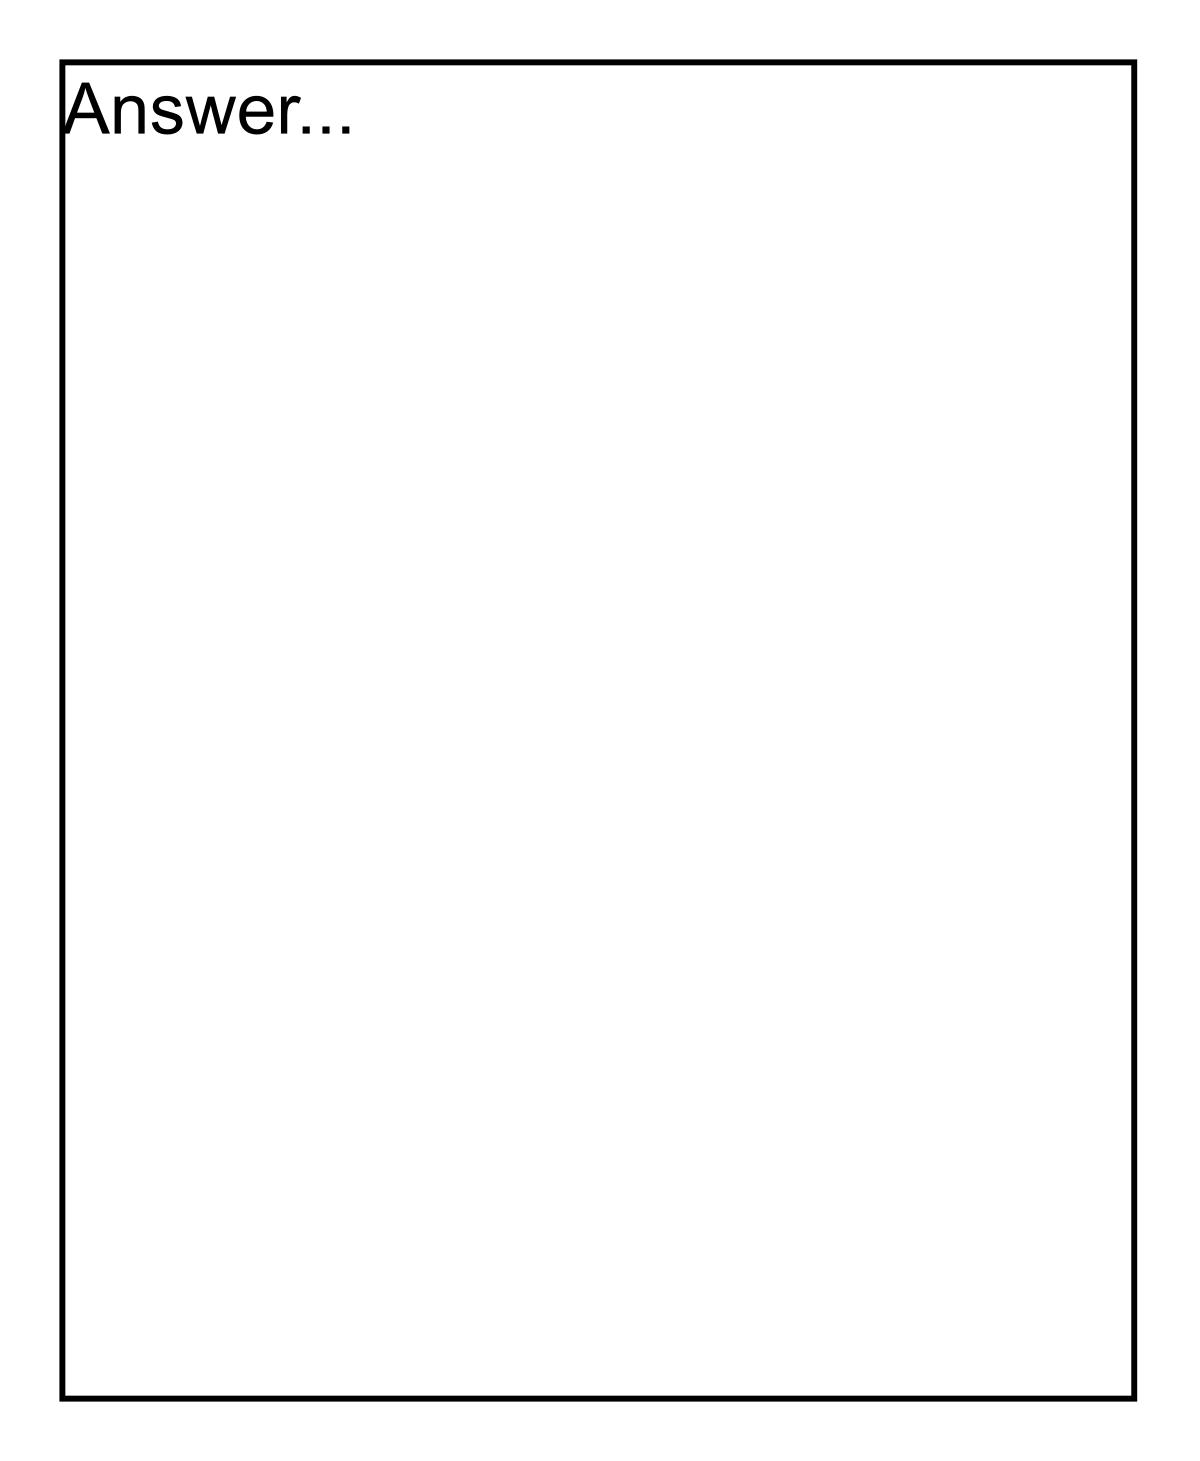
\includegraphics[width=0.5\textwidth]{Images/chapter_20/section_5490973346103296/5131946282582016.png}
 \caption{The class diagram of the Answer class}
\end{figure}

\textbf{R2:} Users should be able to post new questions and add answers to open questions.
\\
\textbf{R4:} A user can upvote, downvote, and add comments to a question or answer. However, they can only upvote a comment.

\subsubsection{Comment}\label{0UpcIEhDJ6vMZUUGsl4WG}
\\
The \texttt{Comment} class refers to an opinion or remark provided by a user on either a question or an answer. It can only be upvoted and flagged, but not downvoted.
\\
The UML representation of the class is shown below:

\begin{figure}[htbp]
 \centering
 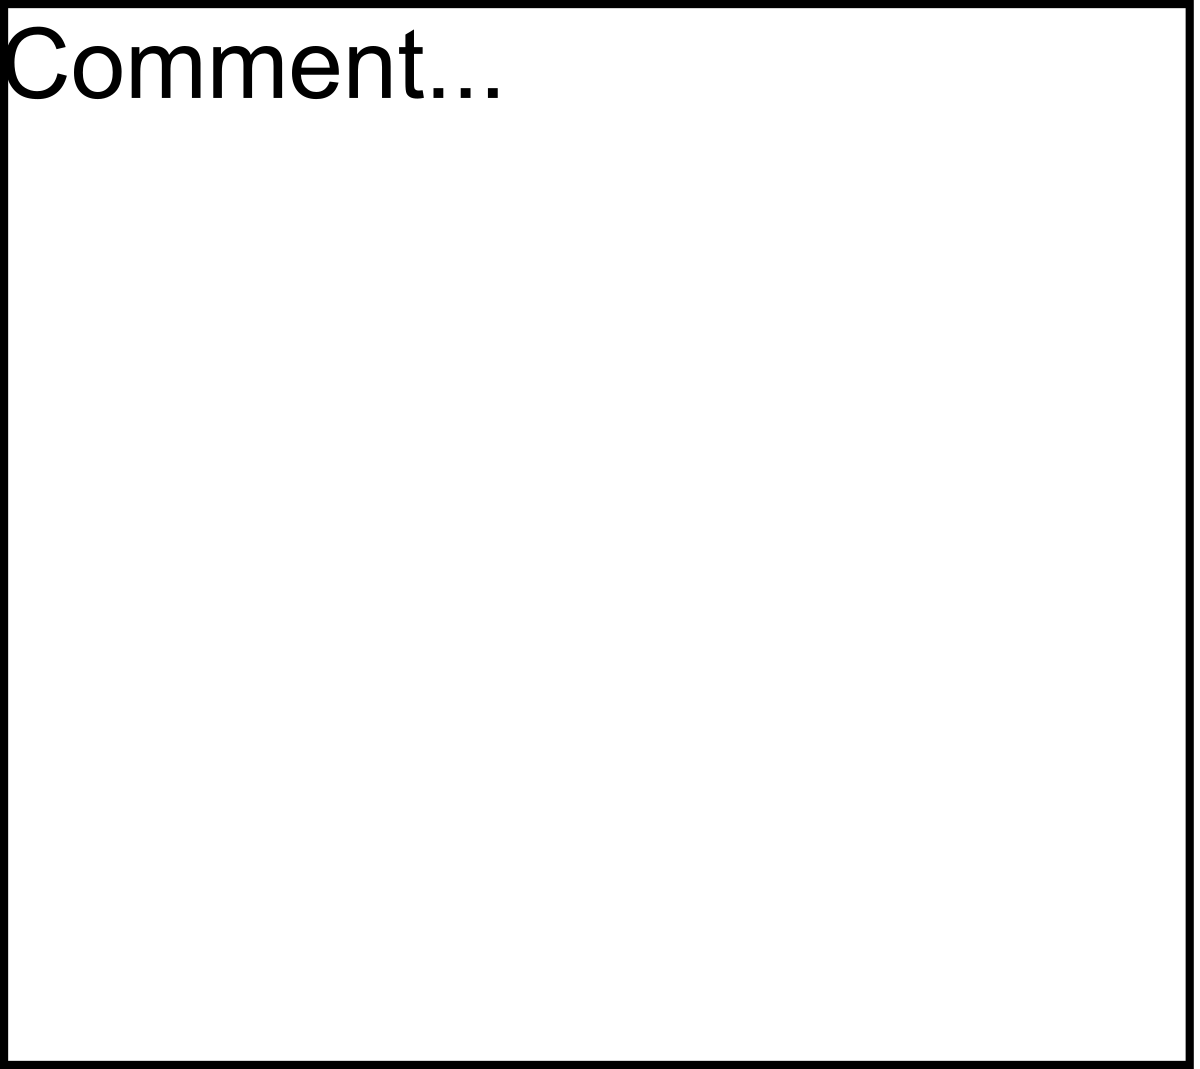
\includegraphics[width=0.5\textwidth]{Images/chapter_20/section_5490973346103296/5239225182322688.png}
 \caption{The class diagram of the Comment class}
\end{figure}

\textbf{R4:} A user can upvote, downvote, and add comments to a question or answer. However, they can only upvote a comment.

\subsubsection{Bounty}\label{xBXtMfEwduQ5v67-Sr9aw}
\\
The \texttt{Bounty} class refers to an award of granting reputation points on a question to attract more attention from other users. It will have an expiry date of seven days and must stay on for at least one day.
\\
The class diagram of the \texttt{Bounty} class is shown below:

\begin{figure}[htbp]
 \centering
 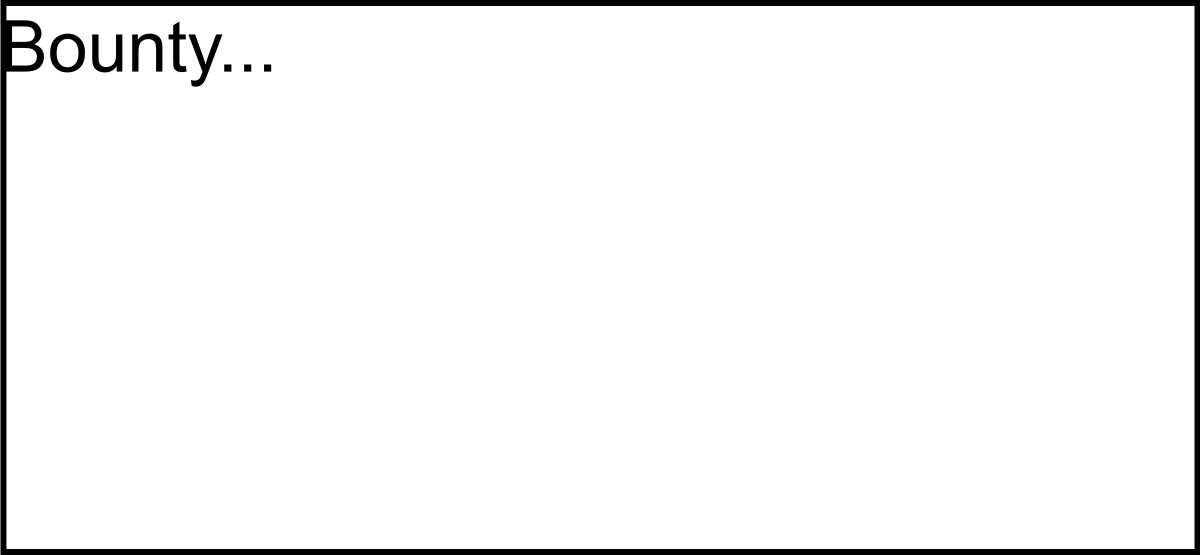
\includegraphics[width=0.5\textwidth]{Images/chapter_20/section_5490973346103296/4565804282806272.png}
 \caption{The class diagram of the Bounty class}
\end{figure}

\textbf{R6:} Users can add a bounty to their question to attract more answers.

\subsubsection{Badge}\label{OzAq7Vny0jcL7yYo0S_KO}
\\
The \texttt{Badge} class refers to badges on a user's profile that show a reputation-worthy user.
\\
The class diagram of the \texttt{Badge} class is shown below:

\begin{figure}[htbp]
 \centering
 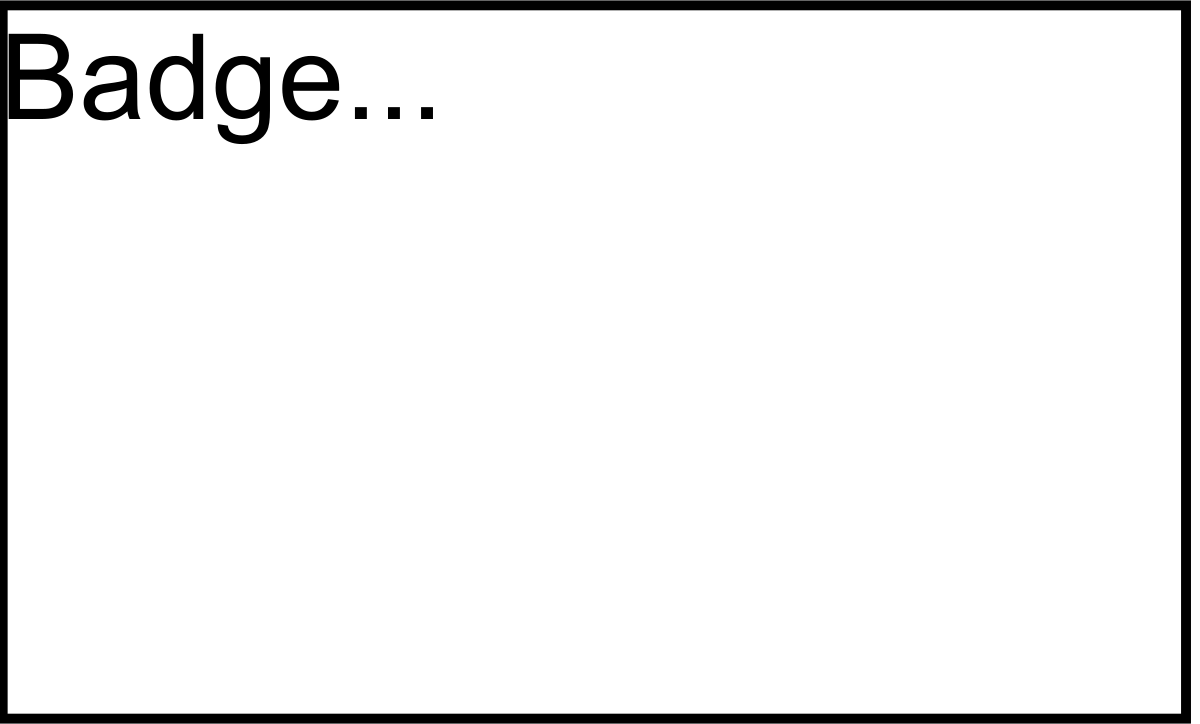
\includegraphics[width=0.5\textwidth]{Images/chapter_20/section_5490973346103296/5967479694426112.png}
 \caption{The class diagram of the Badge class}
\end{figure}

\textbf{R9:} Users can earn badges for helpful answers or comments.

\subsubsection{Tag and tag list}\label{swkpSyiAJ-FnCDXknDch3}
\\
The \texttt{Tag} and \texttt{TagList} classes represent the keywords or labels that categorize questions. The
\texttt{TagList} class contains a key-value pair to keep track of the tag count.
\\
The class diagram for these two classes is provided below:

\begin{figure}[htbp]
 \centering
 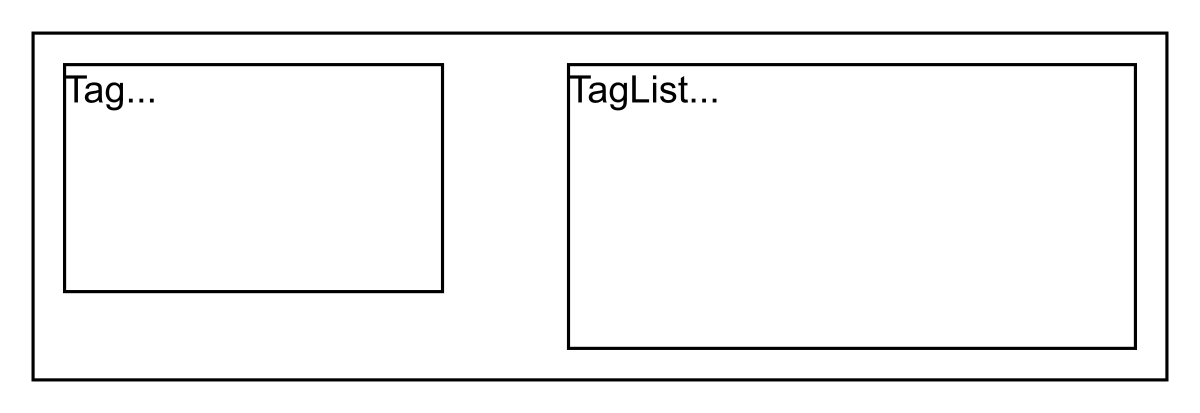
\includegraphics[width=0.5\textwidth]{Images/chapter_20/section_5490973346103296/4810780397404160.png}
 \caption{The class diagram of the Tag and TagList classes}
\end{figure}

\textbf{R10:} Users can add tags to their questions. A tag is a word or phrase describing the question's topic.
\\
\textbf{R11:} The system should also be able to determine the most popular tags used in questions.

\subsubsection{User}\label{MaU8M_jGuOX29FKrU1Rt3-2}
\\
The \texttt{User} class is Stack Overflow's main class and is responsible for various operations, such as creating, answering, and flagging questions, voting to delete or close questions, and more.
\\
The \texttt{User} class is the parent class of the following two classes:

\begin{itemize}
\item
\protect\phantomsection\label{5INmAAQOlk7wPjytOmQ3E}
\texttt{Admin}
\item
\protect\phantomsection\label{-kOy35BNY1DhFCC9u_VSC}
\texttt{Moderator}
\end{itemize}
\\
The details of these are provided below:

\begin{figure}[htbp]
 \centering
 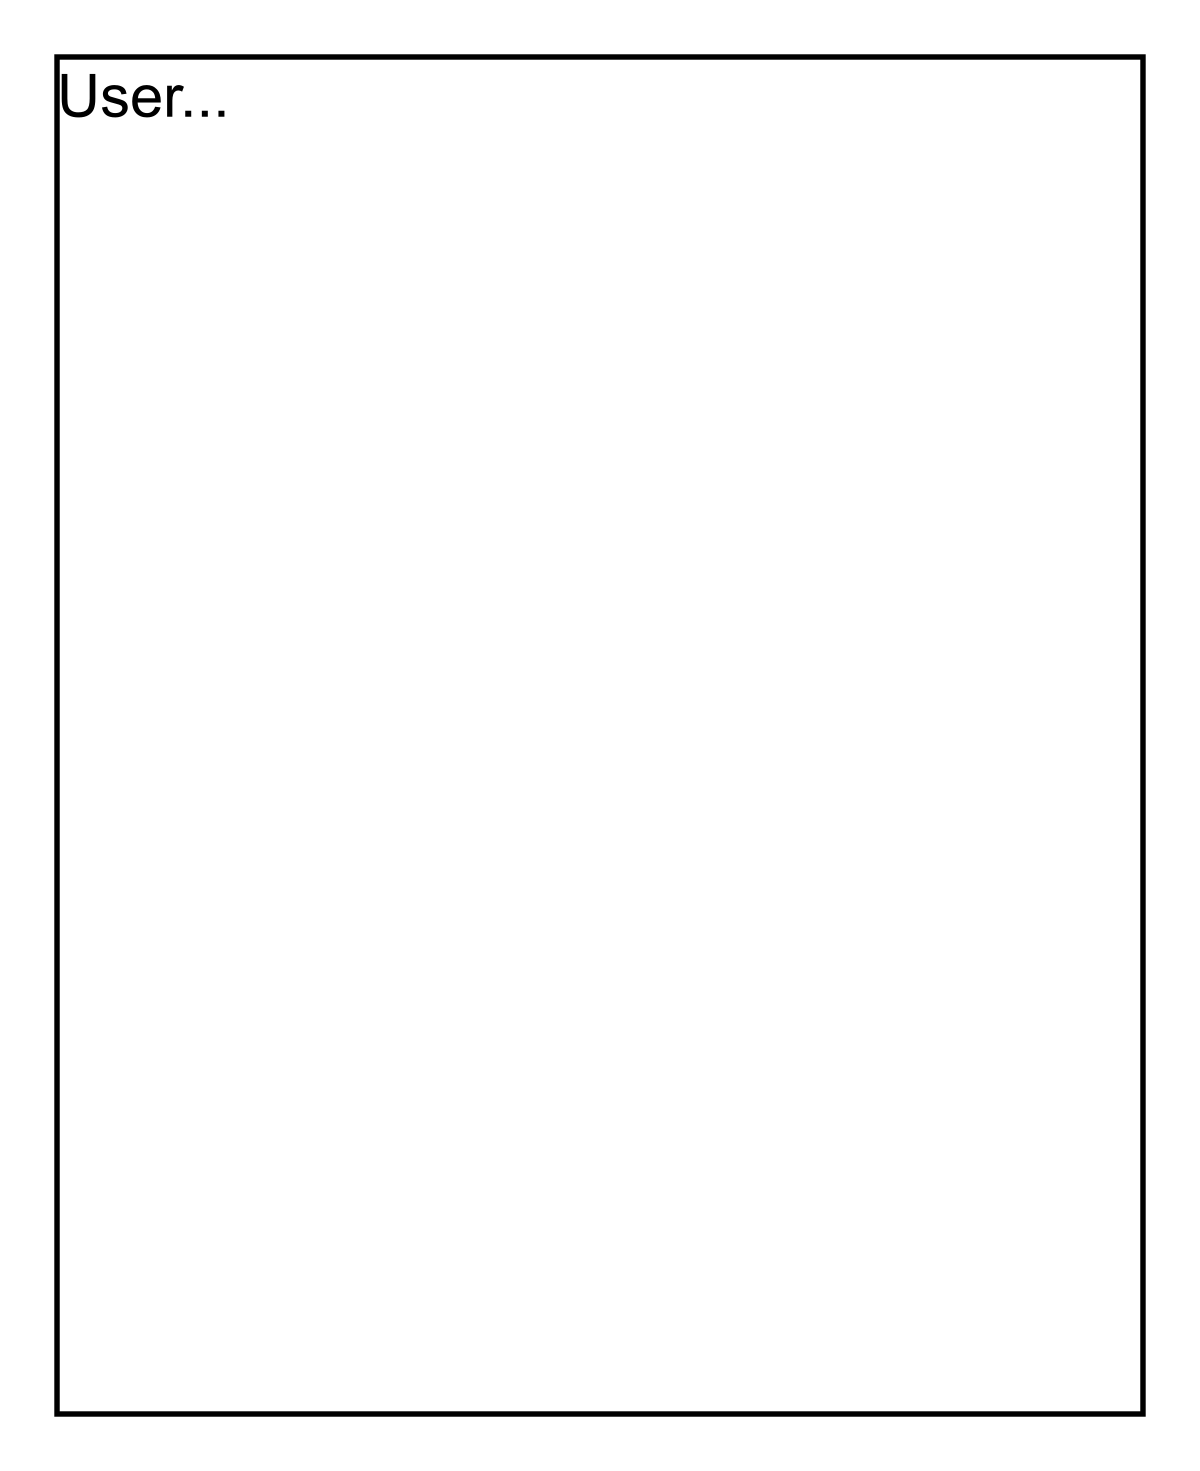
\includegraphics[width=0.5\textwidth]{Images/chapter_20/section_5490973346103296/5636509737549824.png}
 \caption{The class diagram of the User class}
\end{figure}

\paragraph{Admin}\label{lGNyEyQ5HBSPNzQvjs6QK}
\\
The \texttt{Admin} is responsible for performing operations such as blocking or unblocking users.
\\
\paragraph{Moderator}\label{vFS6pX3t7brg_PA3DsPIq}
\\
The \texttt{Moderator} performs operations such as closing, deleting, restoring, and reopening questions.
\\
The class diagram of these classes is provided below:

\begin{figure}[htbp]
 \centering
 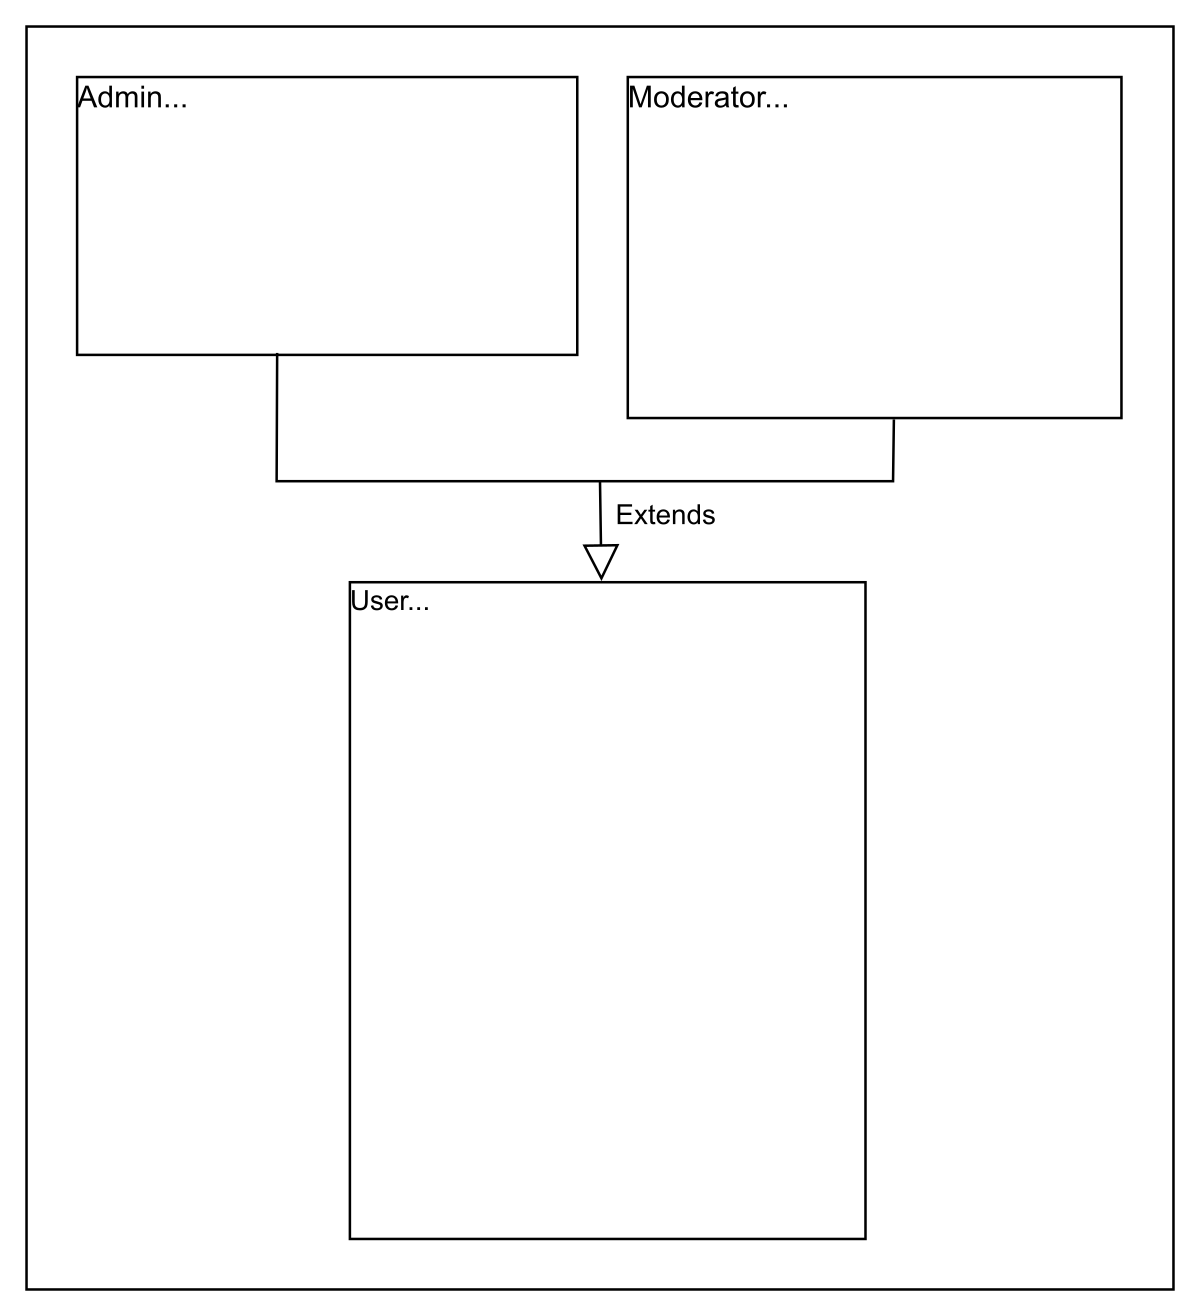
\includegraphics[width=0.5\textwidth]{Images/chapter_20/section_5490973346103296/5645237190787072.png}
 \caption{The class diagram of User and its child classes}
\end{figure}

\textbf{R2:} Users should be able to post new questions and add answers to an open question.
\\
\textbf{R4:} A user can upvote, downvote, and add comments to a question or answer. However, they can only upvote a comment.
\\
\textbf{R7:} Moderators can close questions, restore deleted ones, and delete answers in addition to all the actions available to regular users.

\subsubsection{Notification}\label{UhZSkr_T-ji6-tul56ch2}
\\
The \texttt{Notification} class will send a notification within the Stack Overflow platform whenever a new answer is added to a question asked by a user.
\\
The UML representation of the class is shown below:

\begin{figure}[htbp]
 \centering
 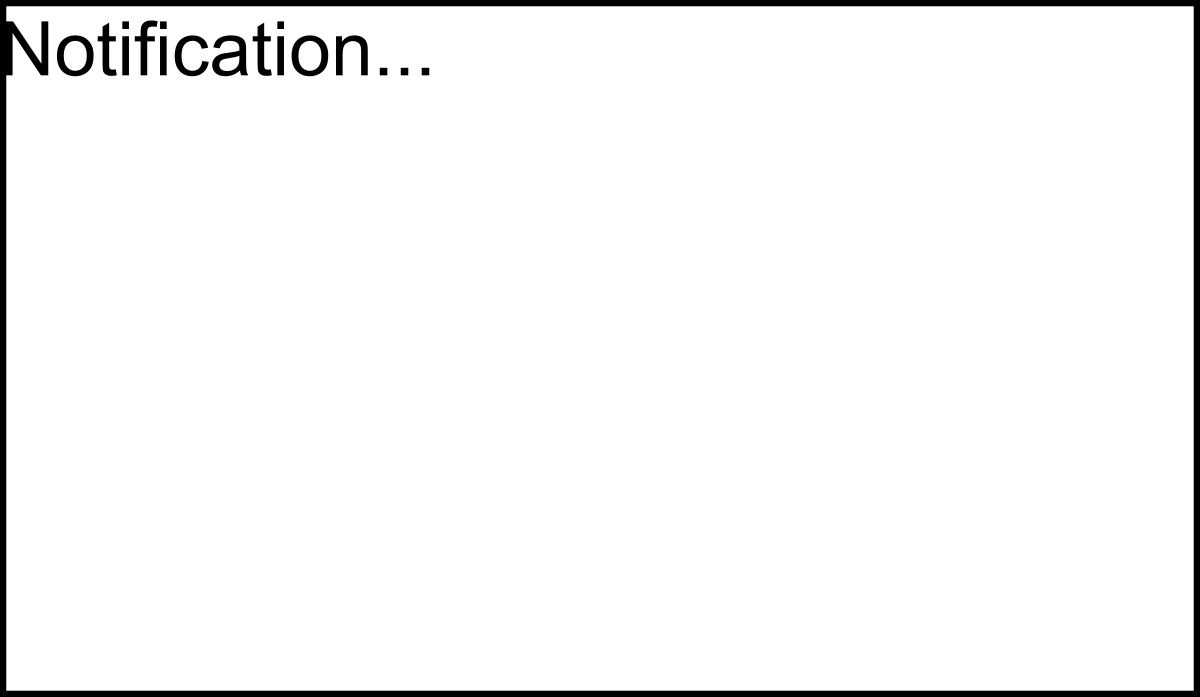
\includegraphics[width=0.5\textwidth]{Images/chapter_20/section_5490973346103296/5687523508748288.png}
 \caption{The class diagram of the Notification class}
\end{figure}

\textbf{R8:} The system should notify the user whenever there has been an interaction with them, such as the user's question receiving an answer, earning a badge, or someone upvoting or downvoting their post.

\subsubsection{Search interface}\label{YDQhuZ6auR1qtkJ9lVyTk}
\\
The \texttt{Search} interface allows users to search for a particular question using tags, usernames, and a string of words.
\\
The UML representation of the interfaces is shown below:

\begin{figure}[htbp]
 \centering
 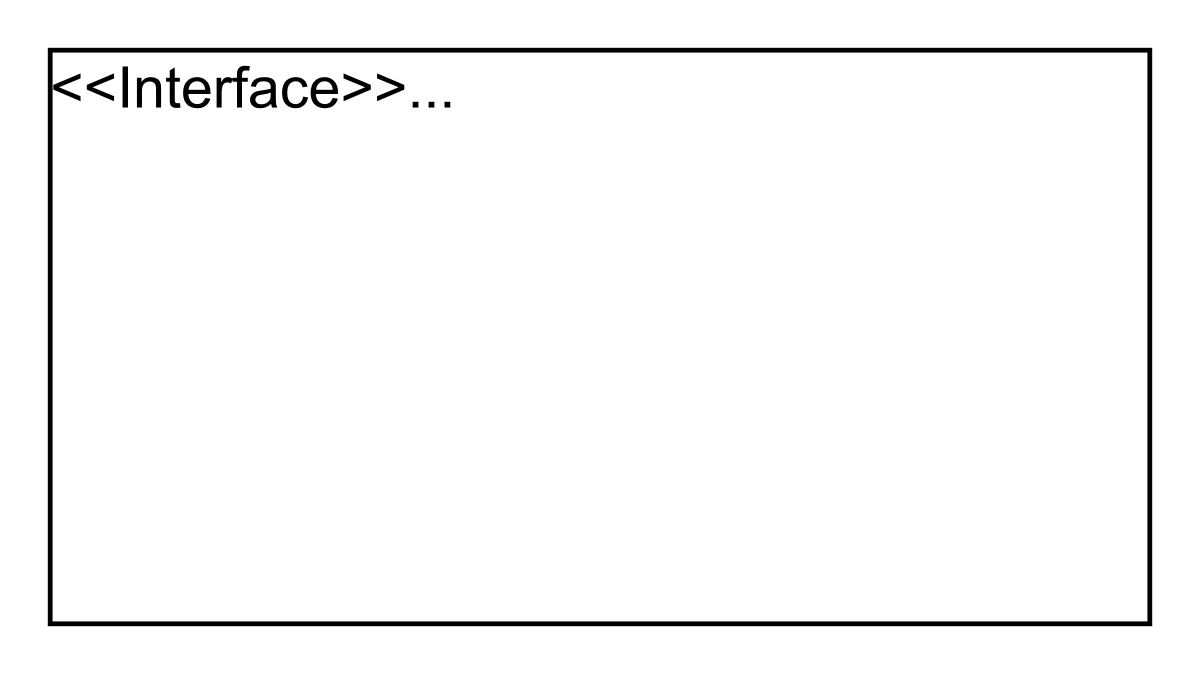
\includegraphics[width=0.5\textwidth]{Images/chapter_20/section_5490973346103296/5256430398341120.png}
 \caption{The class diagram of the Search interface}
\end{figure}

\textbf{R1:} Any guest can view and search questions by tag, username, or word.

\subsubsection{Search catalog}\label{nQm4tZVL6XbCvKn5c7DeE}
\\
The \texttt{SearchCatalog} is the class where the search functionality is implemented. The catalog will fetch the questions using either tags, usernames, or a string of words.
\\
The class representation of the \texttt{SearchCatalog} class is provided below:

\begin{figure}[htbp]
 \centering
 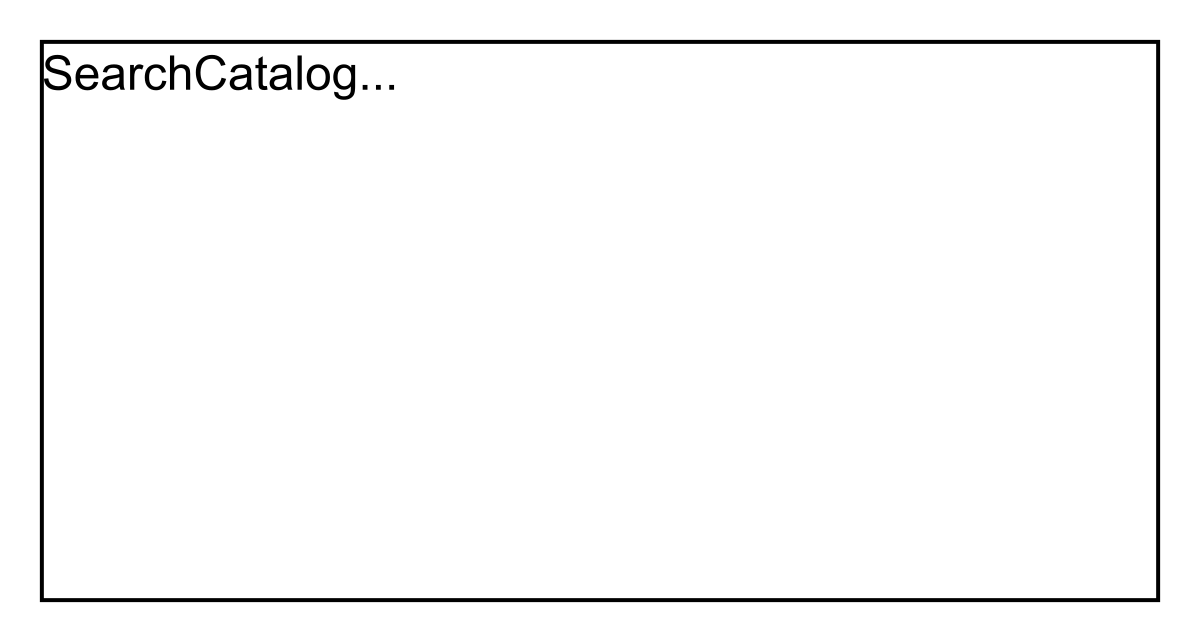
\includegraphics[width=0.5\textwidth]{Images/chapter_20/section_5490973346103296/4586597298077696.png}
 \caption{The class diagram of the SearchCatalog class}
\end{figure}

\textbf{R1:} Any guest can view and search questions by tag, username, or word.

\subsubsection{Enumerations}\label{spPUwOm3kRzPiqkKehu98-2}
\\
The enumerations required in the Stack Overflow design are provided below:

\begin{itemize}
\item
\protect\phantomsection\label{5DywrLQcvebUqutAGjmM3}
\texttt{UserStatus}\textbf{:} The user status tells us about a user's status, whether active or disabled.
\item
\protect\phantomsection\label{mGRKs_o4ff66GeHqfuSxY}
\texttt{QuestionStatus}\textbf{:} The question status describes the status of an existing question, whether it is still active, closed, flagged, or bountied.
\end{itemize}

\begin{figure}[htbp]
 \centering
 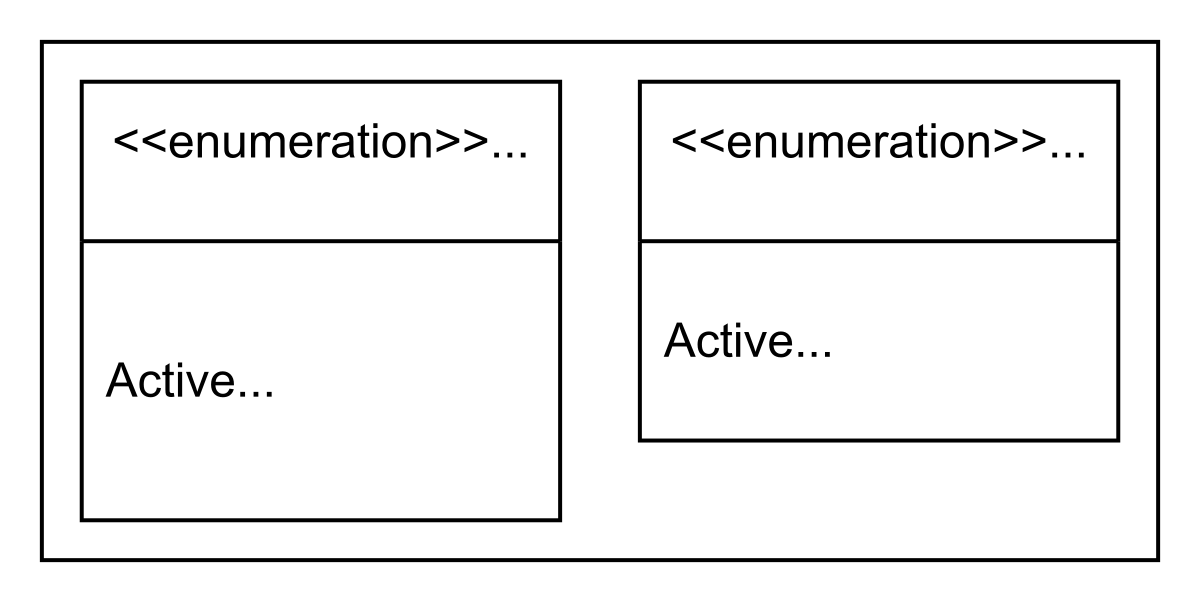
\includegraphics[width=0.5\textwidth]{Images/chapter_20/section_5490973346103296/6616432799252480.png}
 \caption{Enums in Stack Overflow}
\end{figure}

\subsection{Relationship between the classes}\label{spPUwOm3kRzPiqkKehu98-3}
\\
Now, we will discuss the relationships between the classes we have defined above in our Stack Overflow system.

\subsubsection{Association}\label{Ny9Ee_RthPgGHpXLrmxRf}
\\
The class diagram has the following association relationships:

\begin{itemize}
\item
\protect\phantomsection\label{sK4pBE3FlppdHFq9ZRBb_}
The \texttt{User} class has a one-way association with the \texttt{Question}, \texttt{Comment}, \texttt{Badge}, \texttt{Notification}, and \texttt{Search} classes.
\item
\protect\phantomsection\label{JLW5CvhWS2Nvukum0ekdh}
The \texttt{Guest} class has a one-way association with the \texttt{Search} class.
\item
\protect\phantomsection\label{7iEjg98SVTVUllT9AMVXo}
The \texttt{Answer}, \texttt{Comment}, and \texttt{Question} classes have a one-way association with the \texttt{Notification} class.
\item
\protect\phantomsection\label{Kbi2XXQkxnEYC39gNnNbw}
The \texttt{Question} class has a two-way association with the \texttt{Tag} class.
\end{itemize}

\begin{figure}[htbp]
 \centering
 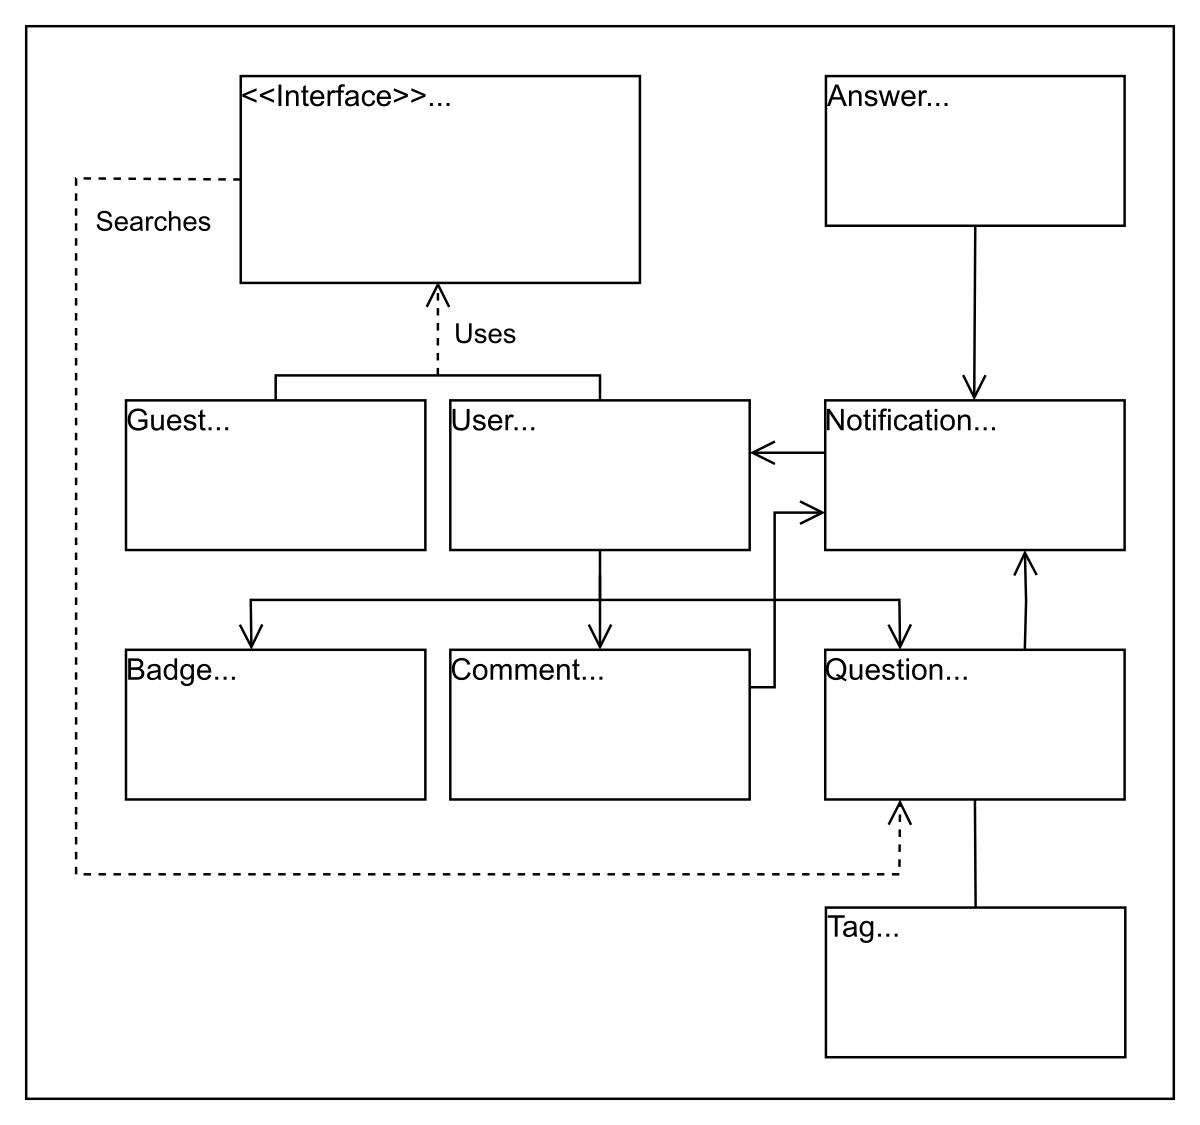
\includegraphics[width=0.5\textwidth]{Images/chapter_20/section_5490973346103296/6592554207150080.png}
 \caption{The association relationship between classes}
\end{figure}

\subsubsection{Composition}\label{spPUwOm3kRzPiqkKehu98-4}
\\
The class diagram has the following composition relationships:

\begin{itemize}
\item
\protect\phantomsection\label{lIWM8Amyl3fvhGt81Q9BN}
The \texttt{Account} class is composed of the \texttt{User} class.
\item
\protect\phantomsection\label{r-1O1xKSInzKeBiNbS_3P}
The \texttt{Question} class is composed of the \texttt{Bounty}, \texttt{Comment}, and \texttt{Answer} classes.
\item
\protect\phantomsection\label{eKWNhOFumNXObkC-6Svyr}
The \texttt{TagList} class is composed of the \texttt{Tag} class.
\end{itemize}

\begin{figure}[htbp]
 \centering
 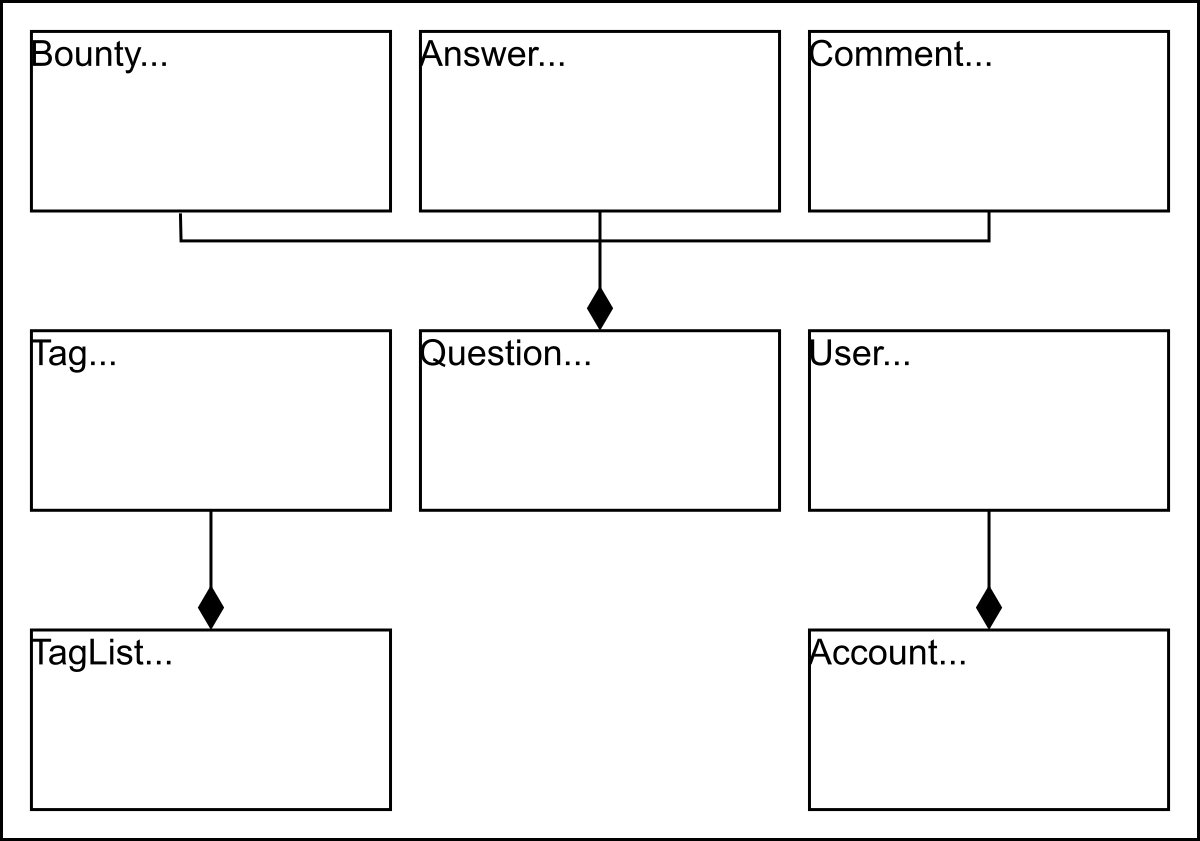
\includegraphics[width=0.5\textwidth]{Images/chapter_20/section_5490973346103296/6615613822992384.png}
 \caption{The composition relationship between classes}
\end{figure}

\subsubsection{Generalization}\label{spPUwOm3kRzPiqkKehu98-5}
\\
The following classes show a generalization relationship:

\begin{itemize}
\item
\protect\phantomsection\label{4DXImm9ge6qpiNJ0l9evJ}
The \texttt{SearchCatalog} class implements the \texttt{Search} interface.
\end{itemize}

\begin{figure}[htbp]
 \centering
 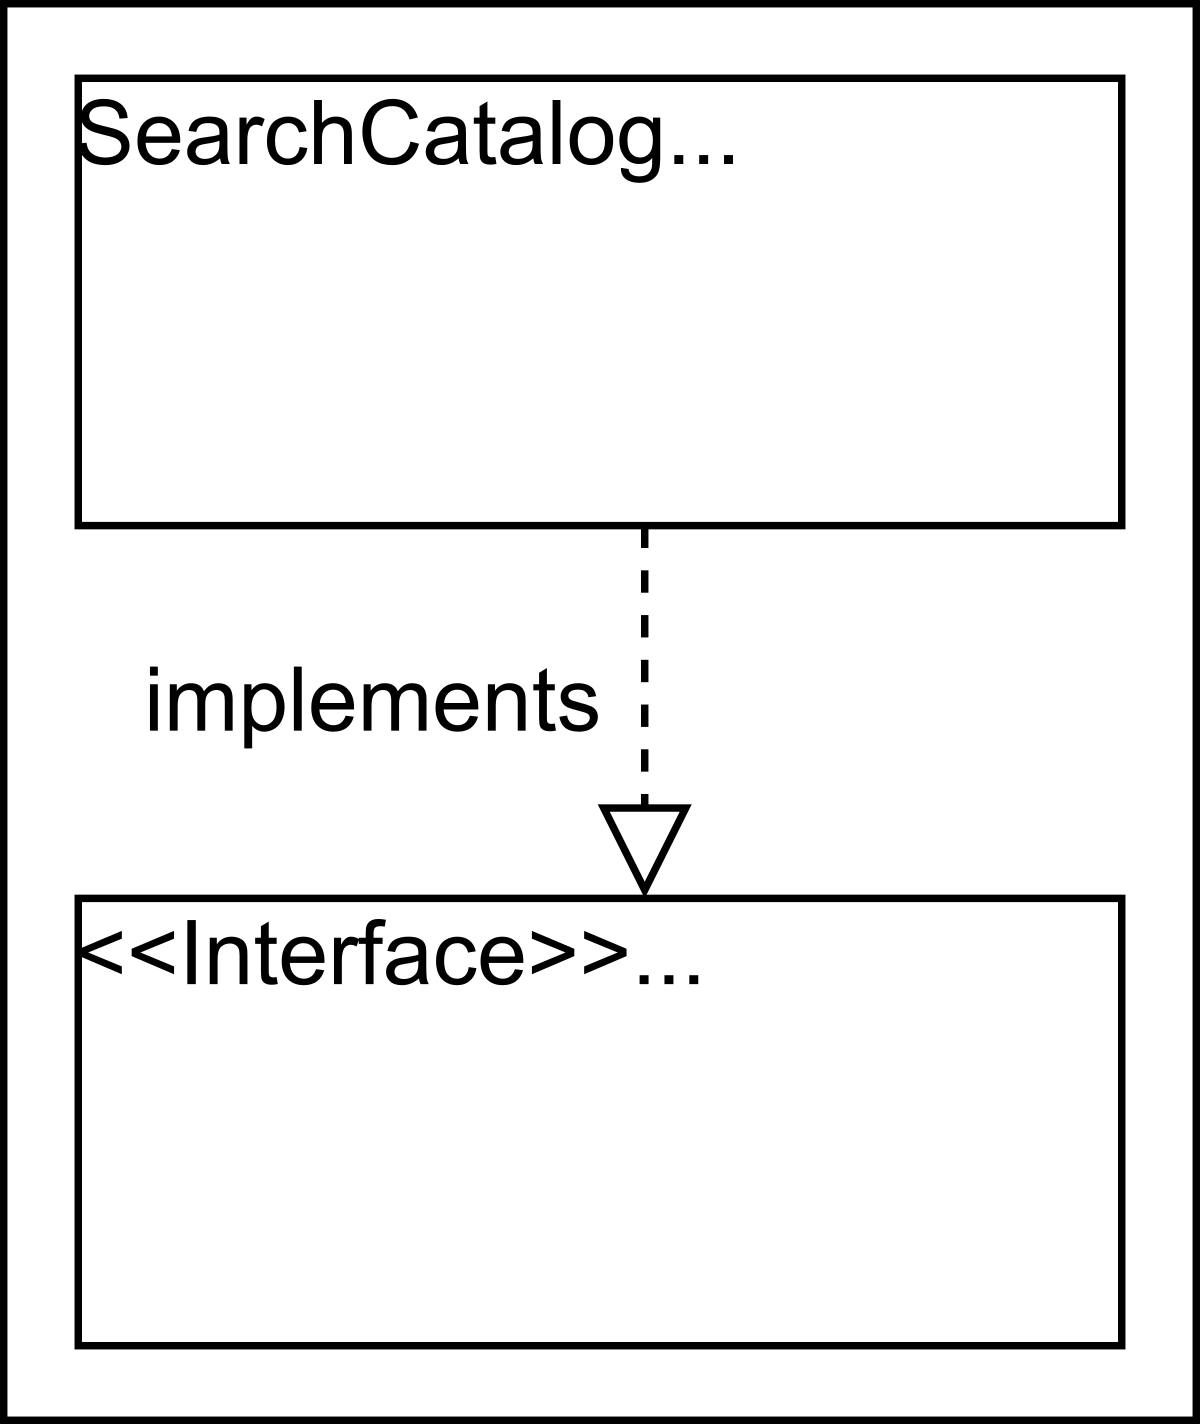
\includegraphics[width=0.5\textwidth]{Images/chapter_20/section_5490973346103296/4792344777064448.png}
 \caption{The generalization relationship between classes}
\end{figure}

\subsubsection{Inheritance}\label{spPUwOm3kRzPiqkKehu98-6}
\\
The following classes show an inheritance relationship:

\begin{itemize}
\item
\protect\phantomsection\label{_GJKGdL2E93QuWD8Lqe65}
Both \texttt{Admin} and \texttt{Moderator} extend the \texttt{User} class.
\end{itemize}
\begin{quote}
\textbf{Note:} We have already discussed the inheritance relationship between classes in the component section above one by one.
\end{quote}
\subsection{Class diagram of Stack Overflow}\label{3sEclHHEhig4Zl_D5AnZy}
\\
In this section, we outline the multiplicity (cardinality) relationships between the main classes in our~Stack Overflow system. For each relationship, we explain the allowed number of instances on each side and the real-world or design rationale behind the connection. Understanding these relationships is key to modeling how different entities interact and collaborate to support key workflows in the system.

\begin{table}[h!]
\centering
\begin{tabular}{|p{3.5cm}|p{3.5cm}|p{3cm}|p{6.5cm}|}
\hline
\textbf{Source} & \textbf{Target} & \textbf{Multiplicity} & \textbf{Reason} \\
\hline
User & Question & 1--0..* & A user can create multiple questions. \\
\hline
Question & User & 1--1 & Each question is created by exactly one user. \\
\hline
User & Answer & 1--0..* & A user can provide multiple answers. \\
\hline
Answer & User & 1--1 & Each answer is associated with exactly one user. \\
\hline
User & Comment & 1--0..* & A user can write multiple comments. \\
\hline
Comment & User & 1--1 & Each comment is posted by one user. \\
\hline
Question & Answer & 1--0..* & A question can have multiple answers. \\
\hline
Answer & Question & 1--1 & Each answer belongs to one question. \\
\hline
Question & Comment & 1--0..* & A question can have multiple comments. \\
\hline
Comment & Question & 0..1--1 & One user posts each comment. \\
\hline
Answer & Comment & 1--0..* & An answer can have multiple comments. \\
\hline
Comment & Answer & 0..1--1 & A comment may be on one answer. \\
\hline
User & Badge & 1--0..* & A user can receive multiple badges. \\
\hline
Badge & User & 0..*--1 & A badge can be awarded to multiple users. \\
\hline
Question & Tag & 1--0..* & A question can have multiple tags. \\
\hline
Tag & Question & 0..*--1 & A tag can be used in multiple questions. \\
\hline
Question & Bounty & 0..1--1 & A question may have one bounty. \\
\hline
Bounty & Question & 1--1 & Each bounty is tied to one question. \\
\hline
User & Notification & 1--0..* & A user can receive multiple notifications. \\
\hline
Notification & User & 1--1 & Each notification is sent to one user. \\
\hline
\end{tabular}
\caption{Entity Relationships and Multiplicities in a Q\&A System}
\label{tab:qa_entity_relationships}
\end{table}


Here's the complete class diagram for Stack Overflow:

\begin{figure}[htbp]
 \centering
 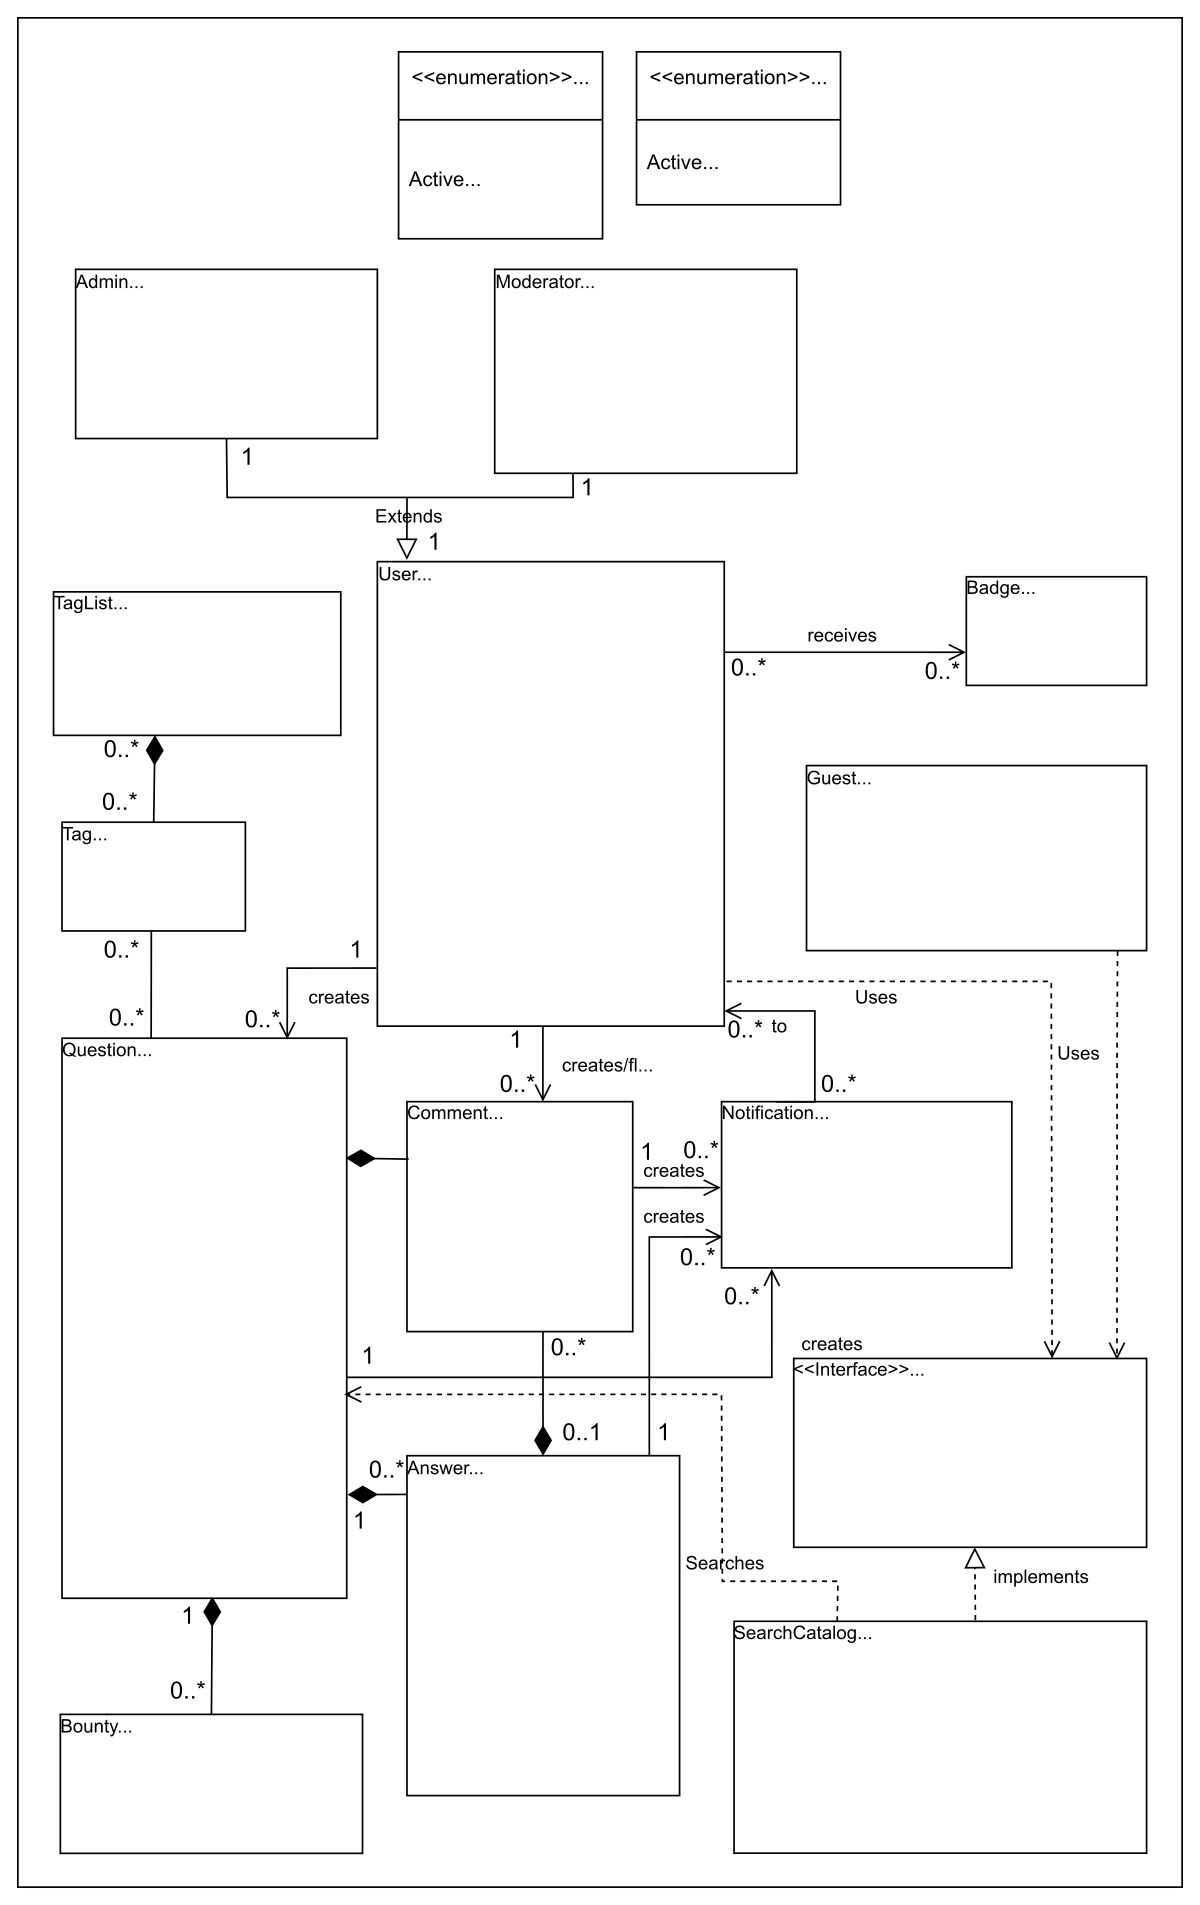
\includegraphics[width=0.5\textwidth]{Images/chapter_20/section_5490973346103296/6731213967327232.png}
 \caption{The class diagram of Stack Overflow}
\end{figure}

\subsection{Design pattern}\label{Yw0AP19fSxPWTnKzxZoSW}
\\
To implement Stack Overflow's core features in a flexible and scalable way, we apply the object-oriented design patterns based on system behavior:

\begin{itemize}
\item
We know that the system notifies users when actions like adding an answer, comment, vote, or badge occur. To model this behavior, we can use the Observer design pattern.
\item
Users can search questions using different criteria, such as tags, keywords, or usernames. We can use the strategy design pattern to handle these interchangeable search methods.
\item
We know the system needs to create different objects, such as questions, answers, comments, and notifications. We can use the Factory Method design pattern to create these objects flexibly and consistently.
\item
We know that users like admins and moderators follow a general workflow, but with some variations in control (e.g., deleting questions, restoring answers). We can use the Template Method design pattern to manage this customizable workflow.
\item
The platform allows dynamic extensions of user capabilities, such as awarding badges or blocking users. Using the Decorator design pattern, we can add such features without modifying existing classes.
\item
We know that comments can be added to both questions and answers. We can use the Composite design pattern to treat these comment structures uniformly.
\item
We know that actions like adding a comment or flagging content could be stored or executed later (e.g., for moderation). We can use the Command design pattern to encapsulate such operations as objects.
\item
The system has different user roles (User, Moderator, Admin), each with specific permissions. We can use role-based access control (RBAC) combined with inheritance to organize access and shared behaviors.
\end{itemize}

\subsection{AI-powered trainer}\label{2j0etUBD4vuDlbOBNDXKu}
\\
At this stage, everything should be clear. If you encounter any confusion or ambiguity, feel free to utilize the interactive AI-enabled widget below to seek clarification. This tool is designed to help you strengthen your understanding of the concepts.

\begin{figure}[htbp]
 \centering
 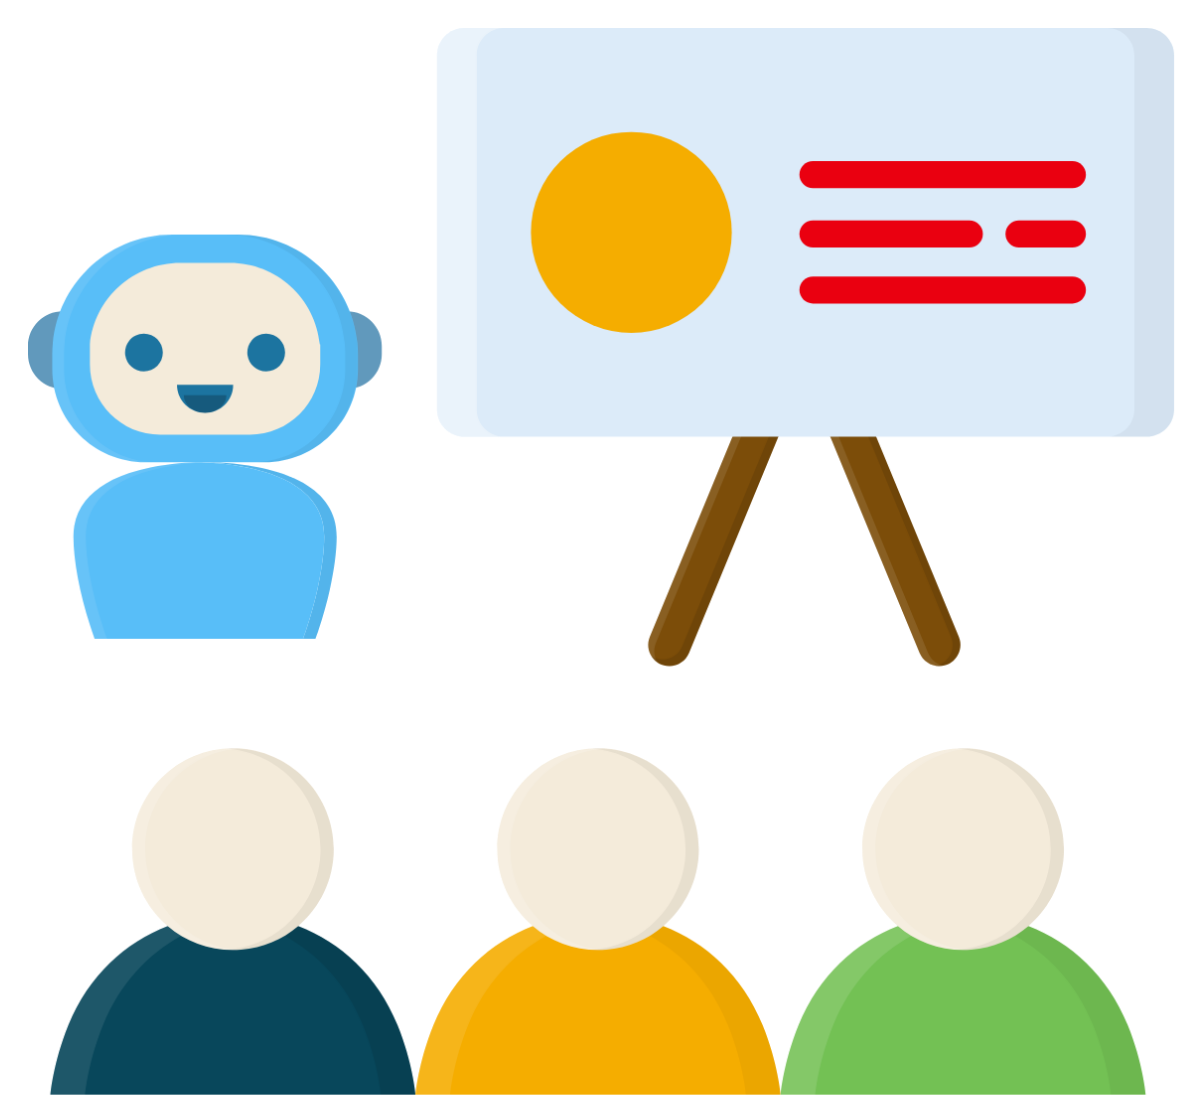
\includegraphics[width=0.15\textwidth]{Images/chapter_20/section_5490973346103296/5176329136635904.png}
 
\end{figure}

\subsection{Additional requirements}\label{3xzU8ULdVQxlzixSxM01k}
\\
The interviewer can introduce some additional requirements in the Stack Overflow system, or they can ask some follow-up questions. Let 's see some examples of additional requirements:

\begin{itemize}
\item
\protect\phantomsection\label{goU49SGlp3NFOlJ7uMc8M}
\textbf{Save questions or answers:} Users can save questions or answers and view them later from the ``Saved'' section in their profile:
\end{itemize}

\begin{figure}[htbp]
 \centering
 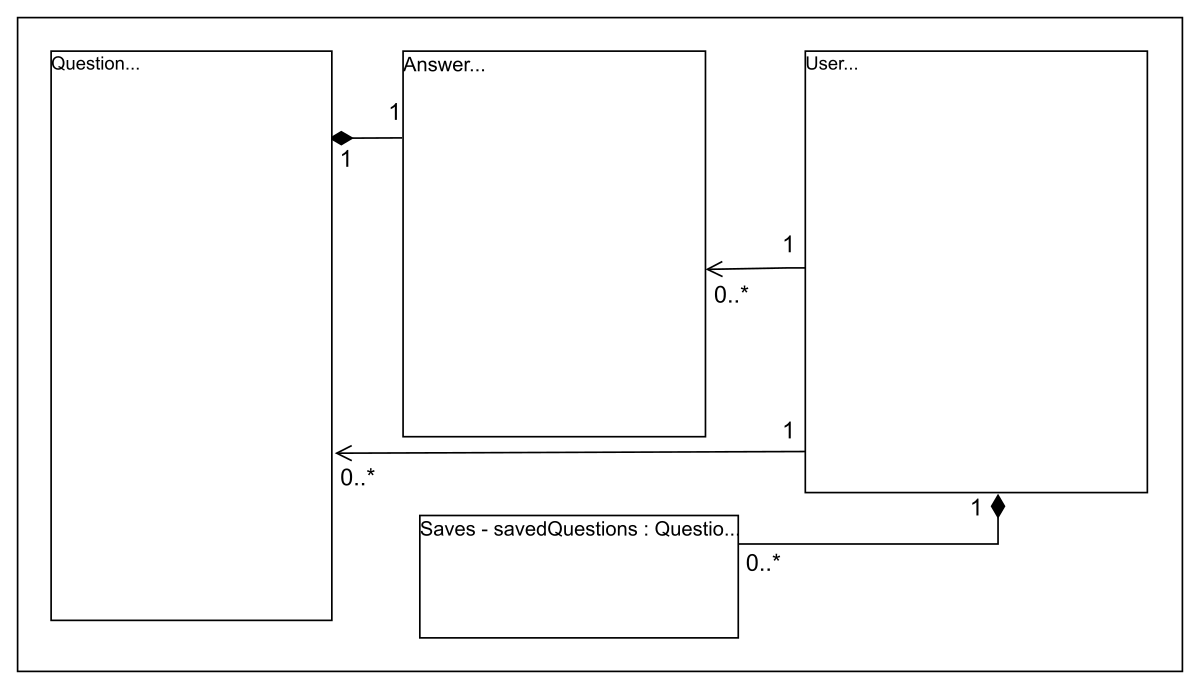
\includegraphics[width=0.5\textwidth]{Images/chapter_20/section_5490973346103296/6048581562531840.png}
 \caption{The class diagram of the save functionality in Stack Overflow}
\end{figure}

We have completed the class diagram of Stack Overflow according to the requirements. In the next lesson, let's design the sequence diagram of Stack Overflow.

% End of section content